\section{Experimental Results}
\label{sec:results}
All numerical comparisons here are descriptive observations on selected
synthetic development instances. They do not establish statistical
significance, population-level effect sizes, or a universal transformation
ranking. Table~\ref{tab:utility} reports the first two incident families
with their distinct model and repetition protocols.
\begin{table}[H]
\centering
\small
\resizebox{\textwidth}{!}{%
\begin{tabular}{llrrrrrr}
\toprule
Family & Condition & Literal & Equal & Unequal & Frequency & Cross-source & Shape \\
\midrule
001 & Raw & 476/476 & 559/559 & 3459/3459 & 20/20 & 326/326 & 476/476 \\
001 & Redaction & 0/476 & 233/559 & 1709/3459 & 0/20 & 0/326 & 0/476 \\
001 & HMAC & 0/476 & 509/559 & 3459/3459 & 15/20 & 276/326 & 0/476 \\
001 & Tokenization & 0/476 & 509/559 & 3459/3459 & 15/20 & 276/326 & 0/476 \\
001 & Format-preserving & 0/476 & 509/559 & 3459/3459 & 15/20 & 276/326 & 476/476 \\
002 & Raw & 190/190 & 300/300 & 2656/2656 & 6/6 & 248/248 & 190/190 \\
002 & Redaction & 0/190 & 52/300 & 1680/2656 & 0/6 & 0/248 & 0/190 \\
002 & HMAC & 0/190 & 300/300 & 2656/2656 & 6/6 & 248/248 & 0/190 \\
002 & Tokenization & 0/190 & 300/300 & 2656/2656 & 6/6 & 248/248 & 0/190 \\
002 & Format-preserving & 0/190 & 300/300 & 2656/2656 & 6/6 & 248/248 & 190/190 \\
\bottomrule
\end{tabular}%
}
\caption{Development representation exposure for annotated identifiers. Counts are retained relationships or shapes over eligible denominators, not a privacy score.}
\label{tab:scalar-exposure}
\end{table}

\begin{table}[H]
\centering
\small
\resizebox{\textwidth}{!}{%
\begin{tabular}{llrrrrr}
\toprule
Family & Condition & Primary valid & Exact RCA & Trigger & Mechanism & Component \\
\midrule
001 & Raw & 5/5 & 5/5 & -- & -- & -- \\
001 & Redaction & 5/5 & 4/5 & -- & -- & -- \\
001 & HMAC & 5/5 & 5/5 & -- & -- & -- \\
001 & Tokenization & 5/5 & 5/5 & -- & -- & -- \\
001 & Format-preserving & 5/5 & 4/5 & -- & -- & -- \\
002 & Raw & 18/18 & 9/18 & 15/18 & 15/18 & 12/18 \\
002 & Redaction & 9/18 & 0/18 & 2/18 & 2/18 & 10/18 \\
002 & HMAC & 18/18 & 1/18 & 1/18 & 1/18 & 13/18 \\
002 & Tokenization & 17/18 & 0/18 & 2/18 & 2/18 & 13/18 \\
002 & Format-preserving & 18/18 & 4/18 & 10/18 & 10/18 & 10/18 \\
\bottomrule
\end{tabular}%
}
\caption{Frozen development RCA. Primary valid shows as-executed coverage; for Incident 002 the RCA columns report the separately labeled 18-valid-per-condition transport-recovered sensitivity view. Incident 001 has no recovery substitution.}
\label{tab:utility}
\end{table}


\paragraph{Identity-dependent Incident 001.}
The frozen GPT-5.6 Luna raw development run obtained 5/5 exact five-label
RCA. Redaction obtained 4/5, HMAC 5/5, tokenization 5/5, and
format-preserving pseudonymization 4/5 on the same five development seeds.
The separate raw-only validation observation was 10/10 exact RCA, but 9/10
\texttt{overall\_correct}: one response cited a nonexistent evidence ID.
There is no matched transformed validation comparison. The
format-preserving development miss localized the defect to request ingress
instead of the oracle operation executor; it did not change the other four
causal dimensions and did not trigger an oracle revision. These small
observations are consistent with the practical value of retaining equality,
not proof that any one deterministic method is generally optimal.

\paragraph{Shape-dependent Incident 002.}
The primary three-trial, six-seed Sol comparison planned 18 logical slots
per condition. It produced 18 valid raw, 9 redaction, 18 HMAC,
17 tokenization, and 18 format-preserving responses. Nine redaction
transport failures and one tokenization timeout remain missing model
responses in that primary analysis, not incorrect RCAs. A separately
authorized one-attempt recovery of exactly those ten cells yielded ten
valid responses and forms the 18-valid-per-condition \emph{sensitivity}
view in Table~\ref{tab:utility}; it does not replace the primary failure
records. In that sensitivity view, raw had 15/18 correct trigger and
mechanism labels and 9/18 exact RCA; format-preserving had 10/18 on each
causal dimension and 4/18 exact; redaction, HMAC, and tokenization had
2/18, 1/18, and 2/18 respectively for trigger/mechanism, with 0/18,
1/18, and 0/18 exact. Component accuracy (12/18 raw, 10/18 redaction,
13/18 HMAC, 13/18 tokenization, 10/18 format-preserving) does not follow
the same ordering. The pattern is directionally consistent with shape
being diagnostically useful, yet format-preserving still missed the
seed-1005 cause in all three logical trials despite its offline invariant
preservation.

\paragraph{Paired temporal Incident 003 v3.}
Table~\ref{tab:temporal-utility} separates overall RCA from correct
mechanism attribution to both roles in the same construction.
\begin{table}[H]
\centering
\small
\resizebox{\textwidth}{!}{%
\begin{tabular}{lrrrrrr}
\toprule
Condition & Valid & Exact RCA & Target mech. & Twin mech. & Paired mech. & Paired exact \\
\midrule
Raw & 8/8 & 7/8 & 4/4 & 3/4 & 3/4 & 3/4 \\
Relative-time & 8/8 & 6/8 & 4/4 & 2/4 & 2/4 & 2/4 \\
Temporal ablation & 8/8 & 4/8 & 4/4 & 0/4 & 0/4 & 0/4 \\
\bottomrule
\end{tabular}%
}
\caption{Incident 003 v3 frozen paired development observations. All three stages used four constructions with target and temporal-twin queries.}
\label{tab:temporal-utility}
\end{table}

\begin{figure}[H]
\centering
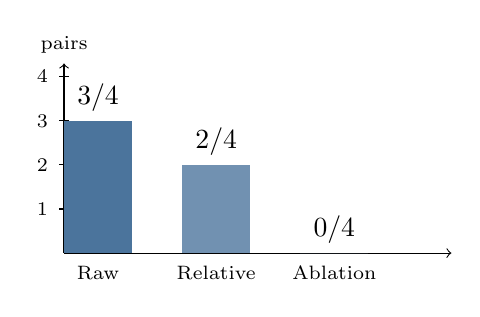
\begin{tikzpicture}[x=1.2cm,y=0.56cm]
\definecolor{diagblue}{RGB}{43,91,139}
\draw[->] (0,0) -- (4.1,0);
\draw[->] (0,0) -- (0,4.3) node[above,font=\scriptsize] {pairs};
\foreach \y in {1,2,3,4} {\draw (-0.05,\y) -- (0.05,\y) node[left,xshift=-4pt,font=\scriptsize] {\y};}
\fill[diagblue!85] (0.00,0) rectangle (0.72,3);
\node[above] at (0.36,3) {3/4};
\node[below,align=center,font=\scriptsize] at (0.36,-0.08) {Raw};
\fill[diagblue!67] (1.25,0) rectangle (1.97,2);
\node[above] at (1.61,2) {2/4};
\node[below,align=center,font=\scriptsize] at (1.61,-0.08) {Relative};
\fill[diagblue!49] (2.50,0) rectangle (3.22,0);
\node[above] at (2.86,0) {0/4};
\node[below,align=center,font=\scriptsize] at (2.86,-0.08) {Ablation};
\end{tikzpicture}
\caption{Paired mechanism discrimination in four frozen Incident 003 v3 development constructions. Raw counts only; no uncertainty bars or equivalence claim.}
\label{fig:paired}
\end{figure}

All eight responses in each stage were valid. Raw evidence yielded 7/8 exact
RCA, with 4/4 target and 3/4 twin mechanism labels correct. Relative-time
yielded 6/8 exact, 4/4 target and 2/4 twin mechanisms. Temporal ablation
yielded 4/8 exact: every target remained correct, every twin was assigned
the target's concurrency mechanism, and no pair was discriminated correctly.
The paired-mechanism sequence 3/4, 2/4, 0/4
(Figure~\ref{fig:paired}) is directionally consistent with the
preregistered development expectation that preserving temporal relations
helps distinguish the two mechanisms. It does not establish equivalence of
raw and relative time, a causal effect size for the provider, or performance
on other incidents. Four pairs and one call per case leave substantial
model-response variability unmeasured.
